\documentclass{article}[12pt]
\usepackage[utf8]{inputenc}
\usepackage[a4paper, margin=1in]{geometry}
\usepackage[english]{babel}
\usepackage{amssymb, amsmath, amsthm} % math symbols
\usepackage{csquotes} % format quote blocks
\usepackage{hyperref} % hyperlinks
\usepackage[table]{xcolor} % tables
\usepackage{graphicx}
\usepackage{multicol}

\hypersetup{
    colorlinks=true,
    linkcolor=black,
    citecolor=black,
    urlcolor=blue,
    pdfborderstyle={/S/U/W 1}
    }

% title
\title{
    Learning Notation: Seminar One \\
    Logic and Proof Techniques
    }
\author{Jack (Quan Cheng) Xie}
\date{March 7, 2022}

% paragraph /indent spacing
\setlength{\parskip}{6pt}
\setlength{\parindent}{0pt}

% mathtools equation numbering
\counterwithin*{equation}{section}
\renewcommand\theequation{\thesection.\arabic{equation}}

% amsthm theorems formatting
\newtheorem{theorem}{Theorem}

\newtheorem{conjecture}{Conjecture}
\newtheorem*{conjecture*}{Conjecture}

\newtheorem{proposition}{Proposition}[section]
\newtheorem*{proposition*}{Proposition} % unnumbered

\newtheorem{corollary}{Corollary}[section]
\newtheorem*{corollary*}{Corollary} % unnumbered

\newtheorem{definition}{Definition}[section]
\newtheorem*{definition*}{Definition} % unnumbered

\newtheorem{exercise}{Exercise}[section]
\newtheorem*{exercise*}{Exercise} % unnumbered

% special symobls
\newcommand{\N}{\mathbb{N}}
\newcommand{\Z}{\mathbb{Z}}
\newcommand{\Q}{\mathbb{Q}}
\newcommand{\R}{\mathbb{R}}
\newcommand{\C}{\mathbb{C}}
\newcommand{\PS}{\mathcal{P}}

% text box for definitions and theorems
\newcommand{\textbox}[1]{\fbox{\parbox{\textwidth}{#1}}}

% bibliography formatting
\makeatletter
\renewcommand{\@biblabel}[1]{$\triangleright$}
\makeatother

\begin{document}

    \maketitle
    
    \section{Mathematical Truth}
        
        \textbf{Discussion.} What is truth? How do we determine the truth? In the context of society, the truth may be determined by:
        \begin{itemize}
            \item 
            Reason or deduction,
            
            \item
            Consensus (e.g. juries, peer-review),
            
            \item
            Authority (e.g. researchers, teachers, judges, politicians),
            
            \item
            Belief or faith.
        \end{itemize}
        
        In mathematics, truth is in some ways very simple. Truth is just a value assigned to a \textbf{statement}.
        
    \subsection{Statements}
        
        \textbox{
        \begin{definition}[Statement]
        \label{def:statement}
            A \textbf{statement} or \textbf{claim} is an expression that is either \textbf{true} ($T$) or \textbf{false} ($F$), but not both. We call $T$ and $F$ \textbf{truth values}.
        \end{definition}
        }
        
        We can use variables to represent a statement. For example:
        \begin{align}
            P &:= 1 + 1 = 2.
            \\
            Q &:= \text{There are infinitely many prime numbers.}
            \\
            R &:= \sqrt{2} \text{ is rational.}
            \\
            S &:= \text{All horses are the same color.}
        \end{align}
        
        For the above statements, $P,\ Q$ are true while $R,\ S$ are false. Not all sentences are statements according to Definition \ref{def:statement}. For example, the truth values of the following sentences cannot be determined, so they are not mathematical statements:
        \begin{align}
            P &:= \text{Hello world!}
            \\
            Q &:= \text{Is $2 + 2 = 4$?}
            \\
            R &:= \text{This statement is false.}
            \\
            S(x) &:= \text{$x$ is even.}
        \end{align}
        
    \subsection{Predicates}
    
        The truth of a statement can depend (or be \textit{predicated}) on a variable. Let $x$ be an integer, and let
        \begin{align}
            P(x) &:= \text{$2x$ is even.}
            \label{eqn:predicate-1}
            \\
            Q(x) &:= \text{$x(x+1)$ is odd.}
            \label{eqn:predicate-2}
        \end{align}

        We call $P(x)$ and $Q(x)$ \textbf{predicates}, and the collection of $x$ the \textbf{universe (or domain) of discourse,} which we describe with a set.

        \textbox{
        \begin{definition}[Set membership]
            \label{def:inf-function}
                A \textbf{set} is a collection of objects, which are called the set's \textbf{members}.
                
                We write $x \in S$ to say that ``$x$ is a member of the set $S$".
        \end{definition}
        }
        
        For example, let $S = \{x, y, z\}$ and assume $a, b, c, d$ are all unique objects (none of them are equal to each other). Then $x \in S = \{x, y, z\}$ is a true statement, and $d \in S = \{x, y, z\}$ is false.
        
        Some sets that are good to know:
        \begin{align*}
            \text{Natural numbers:}\quad &
                \N = \{0, 1, 2, 3, 4, ...\}.
            \\
            \text{Integers:}\quad &
                \Z = \{0, -1, 1, -2, 2, ...\}.
            \\
            \text{Rationals:}\quad &
                \Q = \{..., -1/3, -2, -1/2, -1, 0, 1, 1/2, 2, 1/3, ...\}.
            \\
            \text{Real numbers:}\quad &
                \R = (-\infty, \infty), \quad
                \pi, e, \sqrt{2} \in \R.
        \end{align*}
        
    \subsection{Axioms}
    
        An \textbf{axiom} is a statement that is assumed to be true. An \textbf{axiomatic system} uses axioms, definitions, and deductions to derive the truth values of other statements with \textbf{proofs}.
        
        A statement is \textbf{consistent} in a axiomatic system it does not \textbf{contradict} the other axioms or proven statements. To avoid inconsistencies in a axiomatic system, its axioms should be as few and as simple as possible. Though apparently, constructing a consistent system is \href{https://youtu.be/2YIKpHxitNk?t=192}{more difficult} than it sounds.\cite{rayo-mit} See \href{https://www.youtube.com/watch?v=I4pQbo5MQOs}{more} on \href{https://www.youtube.com/watch?v=O4ndIDcDSGc}{Gödel's incompleteness theorem}.

    \subsection{Proven statements}
    
        \textbf{Theorems, propositions, lemmas,} and \textbf{corollaries} are statements that have or can be \textbf{proven} to be true. \href{https://youtu.be/MXJ-zpJeY3E}{Terence Tao} explains the distinction between them nicely:
        \begin{displayquote}
            ``A \textbf{lemma} is an easily proved claim which is helpful for proving other propositions and theorems, but is usually not particularly interesting in its own right. A \textbf{proposition} is a statement which is interesting in its own right, while a \textbf{theorem} is a more important statement than a proposition which says something definitive on the subject, and often takes more effort to prove than a proposition or lemma. A \textbf{corollary} is a quick consequence of a proposition or theorem that was proven recently.''\cite{tao-book}
        \end{displayquote}
        
    \subsection{Conjectures}
    
        A \textbf{conjecture} is an unproven statement that is believed to be true. \href{https://youtu.be/MxiTG96QOxw}{Goldbach's conjecture} and the \href{https://youtu.be/QKHKD8bRAro}{twin prime conjecture} are two famous examples that are very simple to state, though demonstratively not simple to prove.
        
       \textbox{
       \begin{conjecture}[Goldbach]
            Every even number is the sum of two primes.
       \end{conjecture}
       }
       
       \textbox{
       \begin{conjecture}[Twin prime]
            There are infinitely many primes $p$ where $p + 2$ is also prime.
       \end{conjecture}
       }
            
        Other famous conjectures are the \href{https://youtu.be/d6c6uIyieoo}{ Riemann hypothesis}, the \href{https://youtu.be/YX40hbAHx3s}{ P versus NP problem} and the \href{https://www.youtube.com/watch?v=ZC7wglkBWMM}{continuum hypothesis}. The first two of these are unsolved \href{https://en.wikipedia.org/wiki/Millennium_Prize_Problems}{Millenium Prize Problems}.
            
    
    \section{Predicate Logic}
        
        \renewcommand{\labelenumi}{(\alph{enumi})}
        
        A \textbf{logical operator} (or \textbf{connective}) is applied to one or more statements to create a new statement. We start with \textbf{negation}, which is a \textbf{unary} connective that operates on one statement.
        
    \subsection{Negation and truth tables}
        
        \textbox{
        \begin{definition}[Negation]
            A \textbf{negation} $\neg$ (or $\sim$) is a logical operator on a statement that creates a statement of the opposite truth value. 
        \end{definition}
        }
        
        For example, for a statement $P$, its negation is $\neg P$, which we also call ``not P". We can also negate the negation, $\neg(\neg P)$. Their truth values can be outlined Table \ref{tab:negation}, which is a \textbf{truth table}. A truth table shows all possible truth value combinations of statements or propositional variables.
        
        \begin{table}[!ht]
            \centering
            \begin{tabular}{|c||c|c|}
                \hline
                     $P$ & $\neg P$ & $\neg(\neg P)$
                \\ \hline\hline
                     $T$ & $F$ & $T$
                \\ \hline
                     $F$ & $T$ & $F$
                \\ \hline
            \end{tabular}
            \label{tab:negation}
            \caption{Negation}
        \end{table}
            
            
    \subsection{Logical equivalence}
        
        \textbox{
        \begin{definition}[Logical equivalence]
            Two statements are \textbf{logically equivalent} if they have the same values on the truth table. We express an equivalence between two statements $P$ and $Q$ as $P \equiv Q$. 
        \end{definition}
        }
            
        For example, from Table \ref{tab:negation} we can see that $P \equiv \neg(\neg P)$ since they have the same truth values.
        
    \subsection{Conjunction and disjunction}
            
        \textbox{
        \begin{definition}[Conjunction]
            For two statements $P$ and $Q$, we define their \textbf{conjunction} $P \land Q$ as a statement that is true if both $P$ and $Q$ are true, and false otherwise.    
        \end{definition}
        }
        
        \textbox{
        \begin{definition}[Disjunction]
            We define their \textbf{disjunction} $P \lor Q$ as a statement that is true if either $P$ is true or $Q$ is true, or both are true.
        \end{definition}
        }
    
        We also call $\land$ the ``and" operator and $\lor$ the ``or" operator. The truth table is as follows:
        \begin{table}[!ht]
            \centering
            \begin{tabular}{|c|c||c|c|}
                \hline
                     $P$ & $Q$ & $P \land Q$ & $P \lor Q$
                \\ \hline\hline
                     $T$ & $T$ & $T$ & $T$
                \\ \hline
                     $T$ & $F$ & $F$ & $T$
                \\ \hline
                     $F$ & $T$ & $F$ & $T$
                \\ \hline
                     $F$ & $F$ & $F$ & $F$
                \\ \hline
            \end{tabular}
            \caption{Conjunction and disjunction}
            \label{tab:junctions}
        \end{table}
        
        For statements $x, y, z,$ the following equivalences can be verified with truth tables:
        \begin{align}
            \text{Commutativity:}\quad&&
                x \land y
                \equiv
                y \land x,
                \quad&
                x \lor y
                \equiv
                y \lor x.
            \\\text{Associativity:}\quad&&
                x \land (y \land z)
                \equiv
                (x \land y) \land z,
                \quad&
                x \lor (y \lor z)
                \equiv
                (x \lor y) \lor z.
            \\\text{Distributivity:}\quad&&
                x \land (y \lor z)
                \equiv
                (x \land y) \lor (x \land z),
                \quad&
                x \lor (y \land z)
                \equiv
                (x \lor y) \land (x \lor z).
            \\\text{Identities:}\quad&&
                x \land T \equiv x,
                \quad&
                x \lor F \equiv x.
            \\\text{Annihilators:}\quad&&
                x \land F \equiv F,
                \quad&
                x \lor T \equiv T.
        \end{align}
        
        \begin{exercise}
            Try to verify these algebraic properties with truth tables.
        \end{exercise}
        
    \subsection{De Morgan's laws}
        Two other useful logical equivalences are de Morgan's Laws.
        
        \textbox{
        \begin{theorem}[De Morgan's laws]
            For two statements $P$ and $Q$,
            \begin{align}
                P \land Q &\equiv \neg (\neg P \lor \neg Q), \label{demorg1}\\
                P \lor Q  &\equiv \neg (\neg P \land \neg Q).
                \label{demorg2}
            \end{align}
        \end{theorem}
        }
        
        We will prove the first result \eqref{demorg1} and leave \eqref{demorg2} as an exercise.
        
        \begin{proof}
            To proof that two statements are equivalent, we just have to show that they have the same values on the truth table.
            
            \begin{table}[!ht]
                \centering
                \begin{tabular}{|c|c||c||c|c||c||c|}
                    \hline
                    (i) & (ii) & (iii) & (iv) &
                    (v) & (vi) & (vii)
                    \\
                         $P$ & $Q$ &
                         $P \land Q$ &
                         $\neg P$ & $\neg Q$ &
                         $(\neg P \lor \neg Q)$ &
                         $\neg(\neg P \lor \neg Q)$
                    \\ \hline\hline
                         $T$ & $T$ & $T$ &
                         $F$ & $F$ & $F$ & $T$
                    \\ \hline
                         $T$ & $F$ & $F$ &
                         $F$ & $T$ & $T$ & $F$
                    \\ \hline
                         $F$ & $T$ & $F$ &
                         $T$ & $F$ & $T$ & $F$
                    \\ \hline
                         $F$ & $F$ & $F$ &
                         $T$ & $T$ & $T$ & $F$
                    \\ \hline
                \end{tabular}
                \caption{First de Morgan's Law}
                \label{tab:de-morgans-law-1}
            \end{table}
            
            It can be seen from Table \ref{tab:de-morgans-law-1} that $p \land Q$ in column (iii) and $\neg(\neg P \lor \neg Q)$ in column (vii) have the same truth values for all value combinations of $P, Q$. Therefore they are logically equivalent by definition.
        \end{proof}
        
        \begin{exercise}
            Prove the second de Morgan's law \eqref{demorg2}, that $P \lor Q  \equiv \neg (\neg P \land \neg Q)$.
        \end{exercise}
    
        
        % \begin{table}[!ht]
        %     \centering
        %     \begin{tabular}{|c|c|c|}
        %         \hline
        %          x  &   y   &   z
        %          \\\hline
        %          T  &   T   &   T
        %          \\\hline
        %          T  &   T   &   F
        %          \\\hline
        %          T  &   F   &   T
        %          \\\hline
        %          T  &   F   &   F
        %          \\\hline
        %          F  &   T   &   T
        %          \\\hline
        %          F  &   T   &   F
        %          \\\hline
        %          F  &   F   &   T
        %          \\\hline
        %          F  &   F   &   F
        %          \\\hline
        %     \end{tabular}
        % \end{table}
    
    \subsection{Quantifiers}
        
        \textbf{Quantifiers} connect a sequence of statements from a predicate with conjunction or disjunctions.
        
        \textbox{
        \begin{definition}[Universal quantifier]
            The \textbf{universal quantifier $\forall$} evaluates a conjunction of statements with a predicate $P(x)$ on all elements of $x$ in a set.
            \begin{align}
                \forall x \in \{x_1, x_2, ...\},\; P(x) \ \equiv \ 
                P(x_1) \land P(x_2) \land ...
            \end{align}
        \end{definition}
        }
        
        For the above we read, ``\textbf{For just have to all} $x$ in the set $\{x_1, x_2, ...\}$, $P(x)$ is true." Sometimes we say \textbf{``for every"} or \textbf{``for any"} instead of ``for all"
            
        \textbox{
        \begin{definition}[Existential quantifier]
            The \textbf{existential quantifier $\exists$} creates a disjunction of $P(x)$ for all elements of $x$ in a set.
            \begin{align}
                \exists x \in \{x_1, x_2, ...\},\; P(x) \ \equiv \ 
                P(x_1) \lor P(x_2) \lor ...
            \end{align}
        \end{definition}
        }
        
        For the above we read, ``\textbf{There exists} a $x$ in the set $\{x_1, x_2, ...\}$ where $P(x)$ is true." Sometimes we say \textbf{``there is"} instead of ``there exists."
        
        \begin{exercise}
            The set of natural numbers is $\R$. Consider the following statements:
            \begin{align}
                \text{There exists a real number $a$ where for any real number $x$, $ax = x$.}
                \\
                \text{There exists a real number $b$ where for a any real number $x$, $bx = b$.}
            \end{align}
            Can you rewrite these statements with quantifiers? Are these statements true? If so, what are $a$ and $b$?
        \end{exercise}
        
        \begin{exercise}
            Consider the following statement:
            \begin{align}
                \lim_{x \to p} f(x) = L
                \iff
                \bigg(
                \forall \epsilon > 0, \ 
                \exists \delta > 0, \
                | x - p | < \delta \implies | f(x) - L | < \epsilon
                \bigg)
                .
            \end{align}
            This is called the \textbf{epsilon-delta definition} of limit. Can you restate the definition in words? Can you interpret what it means?
        \end{exercise}
            
    \subsection{Conditional and biconditional statements}
    
        
        \textbox{
        \begin{definition}[Conditional statement]
            For two statements $P$ and $Q$, we can form a new statement
            \begin{align}
                R := \text{If $P$ (is true), then $Q$ (is true)},
            \end{align}
            where $R$ is a true statement if $Q$ is true under the condition that $P$ is true. We can also say that ``$P$ implies $Q$", or ``$Q$ if $P$", or write $P \implies Q$ (or $P \rightarrow Q$).
        \end{definition}
        }
        
        If $P \implies Q$, we call $P$ the \textbf{sufficient condition} for $Q$, and $Q$ the \textbf{necessary condition} for $P$. 
        
        If the reverse implication $Q \implies P$ is true, we can also write $P \impliedby Q$, which we also call the \textbf{converse} of $P \implies Q$. Then we can also say that \textbf{$P$ only if $Q$.}
        
        \textbox{
        \begin{definition}[Biconditional statement]
            For two statements $P$ and $Q$, if both $P \implies Q$ and $P \impliedby Q$, then we say that \textbf{if and only if $P$, then $Q$.} We also call this a biconditional statement, and write it as $P \iff Q$ or $P \longleftrightarrow Q$. A biconditional statement is equivalent to logical equivalence.
        \end{definition}
        }
        
        The truth table for conditional and bi-conditional statements is as follows.
        \begin{table}[!ht]
            \centering
            \begin{tabular}{|c|c||c|c||c|}
                \hline
                     $P$ & $Q$ & 
                     $P \implies Q$ & 
                     $P \impliedby Q$ & 
                     $P \iff Q$
                \\ \hline\hline
                     $T$ & $T$ & 
                     $T$ & $T$ & $T$
                \\ \hline
                     $T$ & $F$ & 
                     $F$ & $T$ & $F$
                \\ \hline
                     $F$ & $T$ & 
                     $T$ & $F$ & $F$
                \\ \hline
                     $F$ & $F$ & 
                     $T$ & $T$ & $T$
                \\ \hline
            \end{tabular}
            \label{tab:cond}
        \end{table}
        
        The third case where $F \implies T$ is true is called ``vacuous truth".
        
        \begin{exercise}
            Show that $P \implies Q$ is logically equivalent to $\neg P \lor (P \land Q)$.
        \end{exercise}
        \begin{exercise}
            Express $P \iff Q$ as negations, conjunctions, and disjunctions of $P$ and $Q$.
        \end{exercise}
        
        % \newpage
        \begin{exercise}
            Which of the following statements are true?
            \begin{multicols}{2}
                \begin{enumerate}
                    \item
                    $x < 3 \implies x \le 4$
                    
                    \item
                    $x < 3 \impliedby x \le 4$
                    
                    \item
                    $x > y \implies x \ge y$
                    
                    \item
                    $x > y \impliedby x \ge y$
                    
                    \item
                    $[(P \implies Q) \land (\neg P)] \implies  (Q \equiv T)$
                    
                    \item
                    $[(P \implies Q) \land (\neg P)] \implies  Q$
                    
                    \item
                    $[(P \implies Q) \land P] \implies Q$
                    
                    % \item
                    % $(|x| < y) \land (y > 0) \iff (x > -y) \land (x < y)$
                    
                    % \item
                    % $(|x| < y) \land (y > 0) \iff (x > -y) \lor (x < y)$
                    
                    % \item
                    % $(|x| > y) \land (y > 0) \iff (x > y) \land (x < -y)$
                    
                    % \item
                    % $(|x| > y) \land (y > 0) \iff (x > y) \lor (x < -y)$
                \end{enumerate}
            \end{multicols}
        \end{exercise}
        
        \subsection{Tautology}
        \textbox{
        \begin{definition}
            A \textbf{tautology} is a statement that is always true.
        \end{definition}
        
        \begin{definition}
            A \textbf{contradiction} is a statement that is always false.
        \end{definition}
            }
            
        For example, $P \lor \neg P$ is a tautology, while $P \land \neg P$ is a contradiction.
        \begin{table}[!ht]
            \centering
            \begin{tabular}{|c|c|c|c|}
                 \hline
                 $P$ & $\neg P$ & 
                 $P \lor \neg P$ &
                 $P \land \neg$ P
                 \\ \hline\hline
                 T & F & 
                 T & F
                 \\ \hline
                 F & T & 
                 T & F
                 \\ \hline
            \end{tabular}
            \caption{A tautology and contradiction}
        \end{table}
            
            % \newpage
            
        \begin{exercise}
            Is each of the following a tautology, contradiction, or neither?
            \begin{multicols}{2}
                \begin{enumerate}
                    \item
                    $(x < 0) \lor (x > 0)$
                    
                    \item
                    $(x < 0) \land (x > 0)$
                    
                    \item
                    $(x < y) \land (x \ge y)$
                    
                    \item
                    $[(P \implies Q) \land (\neg Q)] \implies  \neg P$
                    
                    \item
                    $[(P \lor Q) \land (\neg Q)] \implies  \neg P$
                    
                    \item
                    $(P \land Q) \iff Q$
                    
                    \item
                    $Q \iff (P \lor Q)$
                    
                \end{enumerate}
            \end{multicols}
            
        \end{exercise}
        
        \begin{exercise}
            Verify that the following statements are tautologies.
            
            \begin{multicols}{2}
            \begin{enumerate}
                \item
                $P \iff \neg (\neg P)$
                % Double negation
                
                \item 
                $P \lor Q  \iff \neg (\neg P \land \neg Q)$
                % De Morgan's law
                
                \item
                $P \land Q \iff \neg (\neg P \lor \neg Q)$
                % De Morgan's law
                
                \item\label{eqn:contraposition}
                $(P \implies Q) \iff (\neg Q \implies \neg P)$
                % Contraposition
                
                \item \label{eqn:contradiction}
                $P \iff (\neg P \implies Q) \land (\neg P \implies \neg Q)$
                % Reductio ad absurdum
                
                \item
                $((A \implies B) \land (B \implies C)) \implies (A \implies C)$
                % Syllogism
                
                \item\label{eqn:pf-cases}
                $[(A \lor B) \land (A \implies C) \lor (B \implies C)] \implies C$
                % proof by cases

            \end{enumerate}
            \end{multicols}
            
        \end{exercise}
            
            
            
        % \begin{table}[!ht]
        %     \centering
        %     \begin{tabular}{|c|c||c|c||c|}
        %     \hline
        %          $P$ & $Q$ & 
        %          $\neg P \implies Q$ & 
        %          $\neg P \implies \neg Q$ &
        %          $(\neg P \implies Q) \land (\neg P \implies \neg Q)$
        %     \\ \hline\hline
        %          T & T & 
        %          T & T & T
        %     \\ \hline
        %          T & F & 
        %          T & T & T
        %     \\ \hline
        %          F & T &
        %          T & F & F
        %     \\ \hline
        %          F & F &
        %          F & T & F
        %     \\ \hline
        %     \end{tabular}
        % \end{table}
            
    % \newpage
    \section{Proof Techniques}
        
        
    \subsection{Direct proof}
    
        The most common type of proof is \textbf{direct proof}, where the truth of a statement is derived from direct implications of definitions, axioms, and tautologies.
        
        \textbox{
        \begin{definition}[Odd integer]
            An integer $x$ is odd $\iff$ there exists an integer $y$ where $x = 2y + 1$.
        \end{definition}
        
        \begin{definition}[Even integer]
            An integer $x$ is even $\iff$ there exists an integer $y$ where $x = 2y$.
        \end{definition}
        }
        
        \textbox{
        \begin{proposition}\label{prop:odd-square}
            If the integer $x$ is odd, then $x^2$ is odd.
        \end{proposition}
        }
        
        \begin{proof}(Direct)
            We need to show that there exists integers $a, b$ where $x = 2a + 1 \implies x^2 = 2b + 1$
            \begin{align}
                x = 2a + 1 \implies x^2
                &= (2a + 1)^2 \\
                &= 4a^2 + 4a + 1 \\
                &= 2(2a^2 + a) + 1 \\
                &= 2b + 1, \quad b = 2a(a + 1).
            \end{align}
            Since $a$ is an integer, then $b = 2a(a+1)$ is an integer by closure of addition and multiplication (the sum and product of integers are integers). Then we have shown $x = 2a + 1 \implies x^2 = 2b + 1$ as required.
        \end{proof}
        
        \textbox{
        \begin{theorem}[Pythagoras]
            For any right triangle with edges $abc$ and hypotenuse $c$, we have that
            \begin{align}
                a^2 + b^2 = c^2.
            \end{align}
        \end{theorem}
        }

        \begin{proof}
            
            For any right triangle $abc$ with hypotenuse $c$, we can rotate four identical such triangles to construct a square of edge lengths $a + b$, where another square of length with edge lengths $c$ is inscribed (see example in Figure \ref{tab:pythagoras}).
            \begin{figure}[!ht]
                \centering
                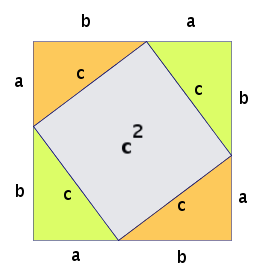
\includegraphics[width=0.5\textwidth]{attachments/1.1-pythagoras.png}
                \caption{Inscribed squares formed from right triangles}
                \label{tab:pythagoras}
            \end{figure}
            
            The area of each of each triangle $abc$ is $\frac{1}{2}ab$ (which can also be proved). The area of the larger square is $(a + b)^2$, and the smaller gray square is $c^2$.
            
            Subtracting the area of the four triangles from the large square, we have that
            \begin{align}
                c^2
                &= (a + b)^2 - \left(4 \frac{1}{2}ab \right)
                \\
                &= (a^2 + 2ab + b^2) - \left(2ab\right)
                \\
                &= a^2 + b^2.
            \end{align}
            Then we have shown that $a^2 + b^2 = c^2$, as required.
        \end{proof}
    
        \begin{exercise}\label{prop:even-prod}
            Prove that if $x$ is an even integer, then $x y$ is even for any integer $y$.
        \end{exercise}
        
        \begin{exercise}
            Prove that if $x$ is an odd integer, then $x^3$ is odd.
        \end{exercise}
        
    \subsection{Proof by cases}
    
        \textbf{Proof by cases} (or \textbf{proof by exhaustion}) is another kind of direct proof, where we exhaust all possible cases of the statement.
        
        \textbox{
        \begin{proposition}
            For any $y \ge 0$, we have that $|x| \le y \implies (-y \le x) \lor (x \le y)$ (or alternatively, $-y \le x \le y$).
        \end{proposition}
        }
        
        \begin{proof}
            The absolute function can be defined as
            \begin{align}
                |x| = \begin{cases}
                    x,  & x \ge 0,
                    \\
                    -x, & x \le 0.
                \end{cases}
            \end{align}
            
            We can show that the implication is true when $x \le 0$ and when $x \ge 0$, which exhausts all cases of $|x| \le y$.
            
            \textbf{Case 1:} If $x \le 0$, then
            \begin{align}
                |x| \le y
                \implies -x \le y
                % \implies -x + x - y \le y + x - y
                % \implies -y \le x
                \implies x \ge -y,
            \end{align}
            which is the first necessary statement in the disjunction.
            
            \textbf{Case 2:} If $x \ge 0$, then
            \begin{align}
                |x| \le y
                \implies x \le y,
            \end{align}
            which is the second necessary statement in the disjunction.
            
            Then we have that
            \begin{align}
                |x| \le y
                \land
                [(x \le 0) \lor (x \ge 0)]
                &\implies (-y \le x) \lor (x \le y)
                \\
                \iff\ 
                |x| \le y
                &\implies (-y \le x) \lor (x \le y),
            \end{align}
            
            since $(x \le 0) \lor (x \ge 0) \equiv T$ is a tautology.
            
        \end{proof}
        
        \begin{exercise}
            Prove that $|x| \ge y \implies (x \le -y) \lor (x \ge y)$.
        \end{exercise}
        
        \begin{exercise}\label{prop:even-sum}
            Prove that if $x, y$ are either both even or both odd, then $x + y$ is even.
        \end{exercise}
        
        \begin{exercise}\label{prop:odd-sum}
            Prove that if $x, y$ are not both even or both odd, then $x + y$ is odd.
        \end{exercise}
        

    \subsection{Proof by contrapositive}
    
        We can also prove statements with \textbf{indirect proofs}, which do not show the truth of the statement from only direct implications. The first type of indirect proof we will look at is \textbf{contrapositive proof}, which proves a conditional statement by proving the contrapositive $\neg Q \implies \neg P$.
        
        This is valid because a conditional statement is logically equivalent to its \textbf{contrapositive} statement, 
        \begin{align}
            (P \implies Q) \iff (\neg Q \implies \neg P),
        \end{align}
        which can be verified with a truth table. Therefore we can prove the original conditional statement by proving the contrapositive instead.
        
        \textbox{
        \begin{proposition}
            For an integer $x$,
            if $x^2 - 6x + 5$ is even, then $x$ is odd.
        \end{proposition}
        }
        
        \begin{proof}(Contrapositive)
            We need to show the \textbf{contrapositive} is true, that
            \begin{align}
                x \text{ is not odd}
                \implies 
                x^2 - 6x + 5 \text{ is not even}.
            \end{align}
            
            If $x$ is not odd then it is even, then there is an integer $a$ where $x = 2a$. Then we have that
            \begin{align}
                x = 2a
                \implies
                x^2 - 6x + 5
                &= (2a)^2 - 6(2a) + 5
                \\
                &= 4a^2 - 12a + 5
                \\
                &= a(4a - 12) + 5
            \end{align}
            
            
            We can show that $a(4a - 12) + 5$ is odd since
            \begin{align}
                & 4a
                &&\text{is even by product of an even integer} \label{eqn:even1}
                \\ \implies
                & 4a - 12
                &&\text{is even by sum of two even integers}  \label{eqn:even2}
                \\ \implies
                & a(4a - 12)
                &&\text{is even by product of an even integer}\label{eqn:even3}
                \\ \implies
                & a(4a - 12) + 5
                &&\text{is odd by sum of two opposite parities}\label{eqn:odd2}
            \end{align}
            
            See exercise \ref{prop:even-prod} for \eqref{eqn:even1} and \eqref{eqn:even3}, exercise \ref{prop:even-sum} for \eqref{eqn:even2}, and exercise \ref{prop:odd-sum} for \eqref{eqn:odd2}. Then we have that
            \begin{align}
                x = 2a \text{ is even}
                \implies
                x^2 - 6x + 5 = a(4a - 12) + 5 \text{ is odd},
            \end{align}
            which is the contrapositive of the original proposition.
        \end{proof}
        
        \textbox{
        \begin{definition}[Informal]
            The derivative of a function $f(x)$ at $x$ can be approximated as
            \begin{align}
                f'(x)
                \simeq \frac{f(x + dx) - f(x)}{dx}
                \simeq \frac{f(x) - f(x - dx)}{dx},
                \ dx > 0.
            \end{align}
            Assume these approximations hold as equalities for an (infinitesimally) small $dx > 0$.
        \end{definition}
        }
        
        \textbox{
        \begin{proposition}[FOC]
            Let $f(x)$ be differentiable. If $f(x^*)$ is the maximum of $f(x)$, then $f'(x^*) = 0$.
        \end{proposition}
        }
        
        \begin{proof}(Contrapositive)
            From the informal definition we can prove the contrapositive of the proposition, which is that
            \begin{align}
                  f'(x^*)
                  = \frac{f(x^* + dx) - f(x^*)}{dx}
                  = \frac{f(x^*) - f(x^* - dx)}{dx}
                  \ne 0
                  \implies f(x^*)
                  \text{ is not the maximum}.
            \end{align}
            
            There are two cases where $f'(x^*) \ne 0$, which are \textbf{1.} $f'(x^*) > 0$ and \textbf{2.} $f'(x^*) < 0$.
            
            \textbf{Case 1.} If $f'(x^*) > 0$, then there is a small $dx > 0$ where
            \begin{align}
                f'(x^*)
                = \frac{f(x^* + dx) - f(x^*)}{dx} > 0
                &\implies
                f(x^* + dx) > f(x^*),
            \end{align}
            which means $f(x^*)$ is not the maximum since there exists a greater value of  $f(\cdot)$.
            
            \textbf{Case 2.} If $f'(x^*) < 0$, then
            there is a small $dx > 0$ where
            \begin{align}
                f'(x^*)
                = \frac{f(x^*) - f(x^* - dx)}{dx} < 0
                &\implies
                f(x^*) < f(x^* + dx),
            \end{align}
            which also means $f(x^*)$ is not the maximum.
            
            Therefore for all cases $f'(x^*) > 0$ and $f'(x^*) < 0$, we have that $f'(x^*) \ne 0$ implies $f(x^*)$ is not the maximum, which is the contrapositive as required.
        \end{proof}
        
        \begin{exercise}
            Prove that for a differentiable function $f(x)$, if $f(x^*)$ is the minimum, then $f'(x^*) = 0$.
        \end{exercise}
        
        \begin{exercise}
            Prove that for any real numbers $x$ and $y$, if $y^3 + yx^2 \le x^3 + xy^2$, then $y \le x$.
        \end{exercise}
        
    \subsection{Proof by contradiction}
        
        Another indirect proof method to show $P$ is true is to show that there is a contradiction from assuming $\neg P$ is true.
        
        This is valid since the statement
        \begin{align}
            P \iff (\neg P \implies Q) \land (\neg P \implies \neg Q)    
        \end{align}
        is a tautology, which says that if $P$ is true, then assuming $\neg P$ is true causes a contradiction from its implications.
        
        
        \textbox{
        \begin{proposition}
            If $x^2$ is even, then $x$ is even.
        \end{proposition}
        }
        
        \begin{proof}(Contradiction)
            Note that the negation of a conditional statement $P \implies Q $ is $P \land \neg Q$:
        \begin{align}
            \neg [P \implies Q]
            &\equiv \neg [\neg P \lor (P \land Q)]
            &&\text{by definition of implication}
            \\
            &\equiv P \land \neg(P \land Q)
            &&\text{by de Morgan's law}
            \\
            &\equiv P \land (\neg P \lor \neg Q)
            &&\text{by de Morgan's law}
            \\
            &\equiv (P \land \neg P) \lor (P \land \neg Q)
            &&\text{by distributivity}
            \\
            &\equiv F \lor (P \land \neg Q)
            &&\text{by contradiction}
            \\
            &\equiv P \land \neg Q
            &&\text{by annihilation}
        \end{align}
        
        Therefore the negation of ``$x^2$ is even \textbf{implies} $x$ is even" is ``$x^2$ is even \textbf{and} $x$ is not even." For the sake of contradiction, suppose $x^2$ is even and $x$ is not even. Then $x$ is odd, and there exists some number $a$ where $x = 2a + 1$. Then
            \begin{align}
                x
                = 2a + 1
                \implies
                x^2
                &= (2a + 1)^2
                \\
                &= 4a^2 + 4a + 1
                \\
                &= 2b + 1, \ b = 2a(a + 1).
            \end{align}
            
            Then $x^2$ is odd, which contradicts the assumption that $x^2$ is even.
        \end{proof}
        
        \textbox{
        \begin{definition}[Rationality]
            A number $q$ is \textbf{rational} if it can be expressed as a quotient of two integers that have no common factors (other than 1).
            \begin{align}
                q \in \Q
                \iff
                \exists\ m, n \in \Z,\quad
                gcd(m, n) = 1,\quad
                q = \frac{m}{n}.
            \end{align}
            
            If $q \in \R$ and $q$ is not rational, then it is \textbf{irrational}.
        \end{definition}
        }
        
        \textbox{
        \begin{proposition}
            The number $\sqrt{2}$ is irrational.
        \end{proposition}
        }
        
        \begin{proof}(Contradiction)
            For sake of contradiction, suppose that $\sqrt{2}$ is rational. Then there exists $p, q \in \Z$ with no common factors where $\sqrt{2} = \frac{p}{q}$. Then we have that
            \begin{align*}
                \sqrt{2} = \frac{p}{q}
                & \implies
                2 = \frac{p^2}{q^2} \\
                & \implies
                p^2 = 2 p^2.
            \end{align*}
            Since $p$ is an integer, then $p$ must be divisible by 2, thus $p = 2m$ for some $m \in \Z$. Then we have that \begin{align*}
                2 q^2 = p^2, p = 2m
                & \implies
                2 q^2 = 4m^2 \\
                & \implies 
                q^2 = 2m^2.
            \end{align*}
            Since $q$ is also an integer, it must also be divisible by 2. Then both $p$ and $q$ are divisible by two, which contradicts the statement that they have no common factors.
        \end{proof}
        
        
        
        
        \textbox{
        \begin{definition}
            A prime number $p$ is a natural number that is only divisible by one and itself. That is, for any other number $n$, the remainder from $p \div n$ is not 0.
            \begin{align}
                p \in \N, \quad
                p \text{ is prime} \iff
                \forall n \in \N, \quad
                2 \le n \le p, \quad
                n \ne p \implies
                n \nmid p.
            \end{align}
        \end{definition}
        }
            
        % \newpage
        
        \textbox{
        \begin{theorem}(Euclid)
            There are infinitely many prime numbers.
        \end{theorem}
        }
        \begin{proof}(Contradiction)
            Suppose for the sake of contradiction that there are finitely many primes. In other words, we can exhaustively list the $n$ many finite primes:
            \begin{align}
                p_1,\ p_2,\ p_3,\ p_4, ...,\ p_n = 2,\ 3,\ 5,\ 7, ...,\ p_n.
            \end{align}
            
            Let $p^*$ be the one plus the product of all finite primes:
            \begin{align}
                p^*
                = 1 + \prod_{i=0}^n p_i
                = 1 + (p_1 \times p_2 \times ... \times p_n).
            \end{align}
            
            The number $p^*$ is not divisible by any of other other primes since $p^* \div p_i$ always has remainder $1$, which is not 0. Then $p^*$ is not divisible by any prime. Then either $p^*$ is a prime that is not included in the list of primes $p_1, p_2, ..., p_n$, or $p^*$ is the product of primes that are not included.
            
            You can always show that a prime number exists outside of any finite set of primes--contradicting the claim that there can exist a finite set containing all primes.
        \end{proof}
        
        \begin{exercise}
            Prove that there are infinitely many natural numbers, supposing that the following statements are true about $\N$, the set of all natural numbers.
            \begin{enumerate}
                \item Zero is a natural number.
                
                \item $\forall n \in \N$, $n + 1$ exists and is a natural number.
                
                \item $\forall n \in \N$, $n+1 \ne 0$.
                
                \item $\forall n, m \in N$, if $n \ne m$, then $n + 1 \ne m + 1$.
            \end{enumerate}
        \end{exercise}
        
        \begin{exercise}
            Prove that there is no smallest positive rational number.
        \end{exercise}
        
        \begin{exercise}
            Prove that $\sqrt{3}$ is irrational.
        \end{exercise}
        
        % \begin{exercise}
        %     Prove that $\sqrt[3]{2}$ is irrational.
        % \end{exercise}
        
        \begin{exercise}
            For $n \in \N,\ n > 1$, show that if $p$ is prime, then $\sqrt[n]{p}$ is irrational.
        \end{exercise}
        
    \subsection{Proof by induction}
    
        The last proof method we will look at is \textbf{induction}, which has to do with statements predicated on a natural number, $P(n),\ n \ge b,\ n \in \N$.
        
        Induction proofs involve two steps:
        \begin{enumerate}
            \item 
            Proof of the \textbf{base case}, that $P(b)$ is true.
            
            \item
            Proof of the \textbf{inductive step,} that $P(k) \implies P(k+1)$. 
        \end{enumerate}
        
        The inductive step allows us to show that
        \begin{align}
            P(b) \Rightarrow P(b+1),\quad
            P(b+1) \Rightarrow P(b+2),
            ... ,\;
            P(n-2) \Rightarrow P(n-1),\quad
            P(n-1) \Rightarrow P(n),
        \end{align}
        which is equivalent of stating that $P(b) \implies P(n)$. Then in conjunction the base case, we have the tautology
        \begin{align}
            P(b) \land [P(b) \implies P(n)]
            \implies
            P(n),
        \end{align}
        which shows that $P(n)$ is true since the sufficient condition is true.
        
        \textbox{
        \begin{proposition}
            For all natural numbers $n \ge 1$, we have that
            \begin{align}
                1 + 2 + 3 + ... + n
                = \sum_{m=1}^n m
                = \frac{n(n + 1)}{2}
            \end{align}
        \end{proposition}
        }
        
        \begin{proof} We will prove this with mathematical induction.
            
            \textbf{Base case.} For $n = \sum_{m=1}^n m = 1$, we have that
            \begin{align}
                \frac{n(n + 1)}{2} = \frac{1(1+1)}{2} = 1.
            \end{align}
            
            \textbf{Inductive step.} We want to show that
            \begin{align}
                \sum_{m=1}^{k} m
                = \frac{k(k+1)}{2}
                % = 1 + 2 + ... + k
                \implies
                \sum_{m=1}^{k+1} m = \frac{(k+1)(k+2)}{2}
                % = 1 + 2 + ... + k + (k + 1)
                .
            \end{align}
            
            We have that
            \begin{align}
                \sum_{m=1}^{k} m = \frac{k(k+1)}{2}
                \implies
                \sum_{m=1}^{k+1} m
                &= [1 + 2 + ... + k] + (k+1)
                = \left[\sum_{m=1}^{k} m \right] + (k+1)
                \\
                &= \left[\frac{k(k+1)}{2}\right] + (k+1)
                =\frac{k(k+1) + 2(k+1)}{2}
                \\
                &=\frac{(k+1)(k+2)}{2}.
            \end{align}
            
            Then it follows by induction that $1 + 2 + 3 + ... + n = \frac{n(n+1)}{2}$.
        \end{proof}
        
        \textbox{
        \begin{definition}[Fibonacci]
            The Fibonacci sequence $\{F_n\}_1^\infty$ follows $F_1 = 1,\ F_2 = 2,$ and for $n > 2$,
            \begin{align}
                F_{n} = F_{n-2} + F_{n-1}
            \end{align}
        \end{definition}
        }
        
        \textbox{
        \begin{proposition}
            The Fibonacci sequence obeys
            \begin{align}
                F_{n+1}^2 - F_{n}^2 - F_{n+1} \cdot F_{n} = (-1)^n
            \end{align}
        \end{proposition}
        }
        
        \begin{proof}
            We will prove this with mathematical induction.
            
            \textbf{Base case.} For $n = 1$, we have that $(-1)^n = (-1)^1 = -1$, and
            \begin{align}
                F_{n+1}^2 - F_{n}^2 - (F_{n+1} \cdot F_{n})
                = F_2^2 - F_1^2 - (F_{n+1} \cdot F_{n})
                = 1 - 1 - (1 \cdot 1)
                = - 1.
            \end{align}
            
            \textbf{Inductive step.} We want to show that
            \begin{align}
                F_{k+1}^2 - F_{k}^2 - (F_{k+1} F_{k}) = (-1)^k
                \implies
                F_{k+2}^2 - F_{k+1}^2 - (F_{k+2} F_{k+1}) = (-1)^{k+1}.
            \end{align}
            
            If $F_{k+1}^2 - F_{k}^2 - F_{k+1} F_{k} = (-1)^k$, then
            \begin{align}
                F_{k+2}^2 - F_{k+1}^2 - (F_{k+2} \cdot F_{k+1})
                &= (F_{k+1} + F_{k})^2 - F_{k+1}^2 - ([F_{k+1} + F_{k}] F_{k+1})
                \\
                &= (F_{k+1}^2 + 2 F_{k} \cdot F_{k+1} + F_{k}^2) - F_{k+1}^2 - (F_{k+1}^2 + F_{k} \cdot F_{k+1})
                \\
                &= F_{k} \cdot F_{k+1} + F_{k}^2 - F_{k+1}^2
                \\
                &= (-1)(F_{k+1}^2 - F_{k}^2 - F_{k} \cdot F_{k+1})
                \\
                &= (-1)(-1)^n = (-1)^{n + 1}.
            \end{align}
            Then the induction proof is complete.
        \end{proof}
        
        
        \begin{exercise}
            Show by induction that for any $n \ge 1$ and any $x \in \R$,
            \begin{align}
                \sum_{m=1}^n x = n x.
            \end{align}
        \end{exercise}
        
        \begin{exercise}
            Show that for any $r \ne 1$,
            \begin{align}
                \sum_{m=0}^n r^m = \frac{1 - r^{n+1}}{1 - r}.
            \end{align}
        \end{exercise}
        
        \begin{exercise}
            Show that for any $n \ge 1$ and any $x \in \R$,
            \begin{align}
                \sum_{m=0}^n m^2 = \frac{n(n-1)(2n-1)}{6}.
            \end{align}
        \end{exercise}
        
        % \begin{exercise}
        %     Show that
        %     \begin{align}
        %         \exists x \in X, P(x)
        %         &\implies
        %         \neg (\forall x \in X, \neg P(x)),
        %         \\
        %         \forall x \in X, P(x)
        %         &\implies
        %         \neg (\exists x \in X, \neg P(x)).
        %     \end{align}
        % \end{exercise}
        
        \begin{exercise}
            Prove the binomial theorem, that for any natural $n \ge 0$,
            \begin{align}
                (x + y)^n
                &= \sum_{k=0}^n \binom{n}{k} x^{n-k} y^k,
                \quad\text{where}\quad
                \binom{n}{k} = \frac{n!}{k! (n-k)!}.
            \end{align}
        \end{exercise}
        
        
        
    \begin{thebibliography}{9}
        
        
        \bibitem{math-apology}
        Hardy, G.H., (1950). \emph{A Mathematician's Apology}. Cambridge University Press.
        \url{http://www.arvindguptatoys.com/arvindgupta/mathsapology-hardy.pdf}
        
        \bibitem{book-of-proof}
        Hammack, Richard, (2018). \emph{Book of Proof, third edition}. Richard Hammack. \url{https://www.people.vcu.edu/~rhammack/BookOfProof/}
        
        \bibitem{mit-compsci-math}
        Leighton, Tom, \& Dijk, Marten. (2010, Fall) \emph{Lecture 1}. 6.042J Mathematics for Computer Science. Massachusetts Institute of Technology: MIT OpenCourseWare. \url{https://youtu.be/L3LMbpZIKhQ}
        
        \bibitem{rayo-mit}
        Rayo, Agustin, (2020). \emph{About this class}, lecture. Paradox and Infinity. MIT Open Learning Library. \url{https://openlearninglibrary.mit.edu/courses/course-v1:MITx+24.118x+2T2020/course}
        
        \bibitem{libretexts-logic}
        Statements and Logical Operators. (2021, September 5). Grand Valley State University. \url{https://math.libretexts.org/@go/page/7039}
        
        \bibitem{tao-notes}
        Tao, Terence. (2003). \emph{Week 1}, lecture notes. Honors Analysis Math131AH. University of California, Los Angeles. \url{https://www.math.ucla.edu/~tao/resource/general/131ah.1.03w/}
        
        \bibitem{tao-book}
        Tao, Terence. (2016). \emph{Analysis I, third edition}. Springer Singapore.
        
    \end{thebibliography}
    % \bibliographystyle{plain}
    % \bibliography{1-sets.bib}
    
\end{document}